\section{Rationaaliluvut}
    \label{rationaaliluvut}
    
    \emph{Rationaaliluvulla} tarkoitetaan lukua $q$, joka voidaan esittää muodossa
    \[
    q=\frac{a}{b}, 
    \]
    missä $a$ ja $b$ ovat kokonaislukuja ja $b\neq 0$. Rationaalilukujen joukkoa
    merkitään symbolilla $\mathbb{Q}$. Rationaaliluvun esitystä osamääränä
    $\frac{a}{b}$ kutsutaan \emph{murtoluvuksi}. Luku $a$ on murtoluvun
    \emph{osoittaja} ja luku $b$ on \emph{nimittäjä}. Kaikki rationaaliluvut
    voidaan esittää murtolukuina, mutta murtoluvut eivät ole ainoa tapa
    rationaalilukujen esittämiseksi . Kaikki rationaaliluvut voidaan myös
    esittää usealla eri tavalla murtolukuna. 
         Rationaalilukujen ja murtolukujen erona on, että rationaaliluvut
    ovat lukujen muodostama joukko, kun taas murtoluvut ovat lukujen esitystapa.
    Vaihtoehtoinen esitystapa rationaaliluvuille on \emph{desimaaliluvut},
    esimerkiksi murtoluku $\frac{1}{2}$ ja desimaaliluku $0,5$
    esittävät samaa rationaalilukua.
    
    \laatikko{
        Murtoluku on osamäärä
        \[
        \frac{a}{b}
        \]
        missä $a,b \in \mathbb{Z}$ ja $b \neq 0$. Jokaisen murtoluvun arvo on
        rationaaliluku ja jokainen rationaaliluku voidaan esittää murtolukuna.
    }
\subsection*{Murtolukujen laskusäännöt}

\begin{esimerkki}
        Murtolukujen yhteenlasku. Laske
        \[
        \frac{1}{2} + \frac{1}{6} + \frac{2}{6}.
        \]
        
        \textbf{Ratkaisu.}
        Lavennetaan nimittäjät samannimisiksi ja lasketaan osoittajat yhteen:
        %lisätäänkö lavennusmerkki? teknisesti hankala? käytetäänkö maailmalla? opiskelijoille kuitenkin tuttu
        \begin{align*}
            \frac{1}{2} + \frac{1}{6} + \frac{2}{6} &=\frac{3\cdot 1}{3\cdot 2} + \frac{1}{6} + \frac{2}{6}\\
            										&=\frac{3}{6} + \frac{1}{6} + \frac{2}{6}\\
           											&= \frac{3+1+2}{6}\\
           											&= \frac{6}{6} = 1.
        \end{align*}
    \end{esimerkki}

\laatikko{
    Jos murtolukujen
    nimittäjät ovat samat, voidaan murtoluvut laskea yhteen laskemalla
    osoittajat yhteen.
    \[
    \frac{a}{c} + \frac{b}{c} = \frac{a+b}{c}
    \]
}

    Murtolukuja, joiden nimittäjät ovat samat, sanotaan \emph{samannimisiksi}.
    Jos yhteenlaskettavien murtolukujen nimittäjät eivät ole samat, murtoluvut
    \emph{lavennetaan} ensin samannimisiksi ja sitten osoittajat lasketaan yhteen.
    Jos siis $\frac{a}{b}$ ja $\frac{c}{d}$ ovat murtolukuja, lasketaan

\laatikko{
    \[
    \frac{a}{b} + \frac{c}{d} = \frac{ad}{bd} + \frac{bc}{bd} = \frac{ad+bc}{bd}
    \]
    Tässä $\frac{a}{b}$ lavennetaan $d$:llä ja $\frac{c}{d}$ lavennetaan
    $b$:llä, jolloin saadaan kaksi samannimistä murtolukua, joiden kummankin
    nimittäjä on yhteenlaskettavien nimittäjien tulo $bd$.
 }    

\begin{esimerkki}
        Murtolukujen kertolaskussa osoittajat ja nimittäjät kerrotaan keskenään.
      \[
        \frac{3}{4}\cdot \frac{6}{5}= \frac{3\cdot 6}{4\cdot 5}= \frac{18}{20}=\frac{9}{10}
        \]
    \end{esimerkki}
\laatikko{
    Murtolukujen $\frac{a}{b}$ ja $\frac{c}{d}$ tulo lasketaan kertomalla lukujen osoittajat ja nimittäjät keskenään:
    \[
    \frac{a}{b}\cdot \frac{c}{d} = \frac{a\cdot c}{b\cdot d} = \frac{ac}{bd}
    \]
}

%\missingfigure{tähän Sampon paperille suunnittelema havainnollistus kertolaskusäännöstä}
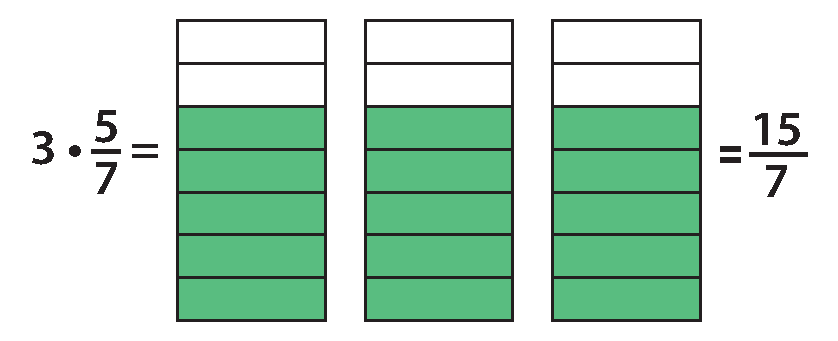
\includegraphics[scale=0.4]{pictures/Kuva3-1-1.pdf}
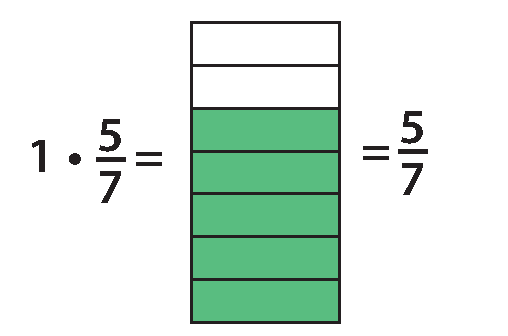
\includegraphics[scale=0.4]{pictures/Kuva3-1-2.pdf}
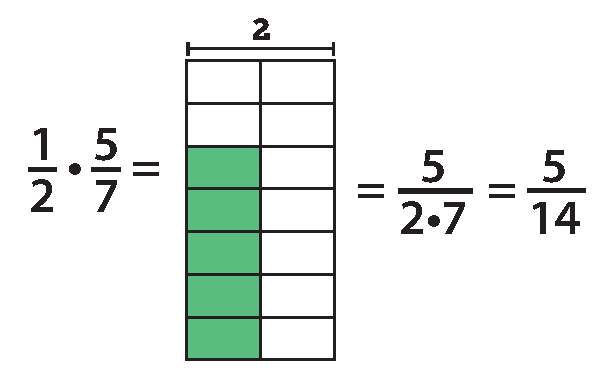
\includegraphics[scale=0.4]{pictures/Kuva3-1-3.pdf}
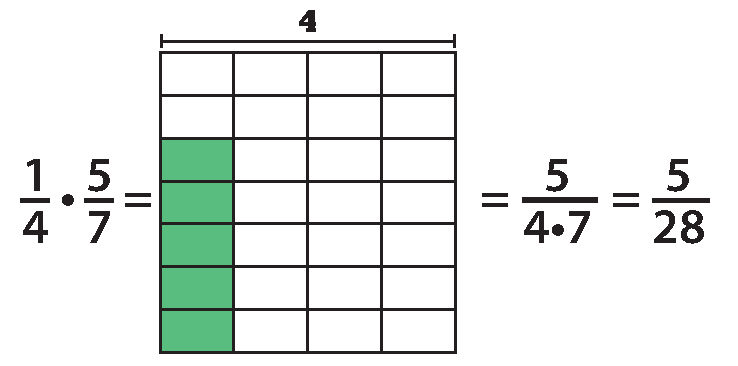
\includegraphics[scale=0.4]{pictures/Kuva3-1-4.pdf}
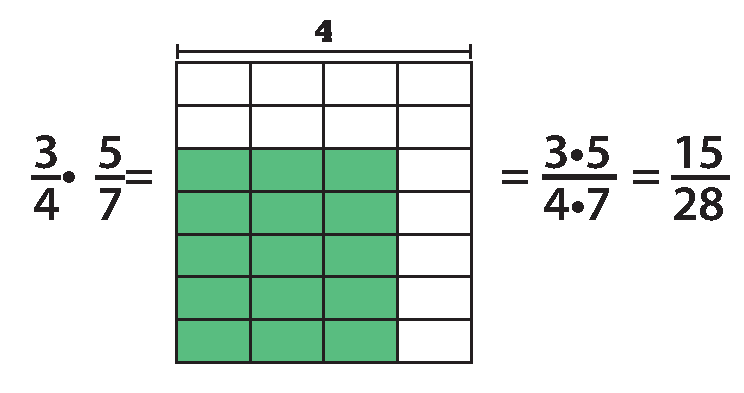
\includegraphics[scale=0.4]{pictures/Kuva3-1-5.pdf}

\begin{esimerkki}
	Luvun $5$ \emph{käänteisluku} on $\frac{1}{5}$, koska
	\[
	 5\cdot \frac{1}{5}=1.
	\]
	Vastaavasti luvun $-\frac{2}{3}$ käänteisluku on $-\frac{3}{2}$, koska
	\[
	 -\frac{2}{3}\cdot (-\frac{3}{2})=1.
	\]

\end{esimerkki}
\laatikko{
    Rationaaliluvun $a$ ($a\neq 0$) \emph{käänteisluku} on  $\frac{1}{a}$, sillä
    \[
    a\cdot \frac{1}{a} = 1.
    \]
    Vastaavasti rationaaliluvun $\frac{a}{b}$ ($a\neq 0$ ja $b\neq 0$) käänteisluku on $\frac{b}{a}$, sillä
    \[
    \frac{a}{b}\cdot \frac{b}{a} = 1.
    \]    

  %  Murtolukujen $p=\frac{a}{b}$ ja $q=\frac{c}{d}\neq 0$ \emph{osamäärä} $p : q$ saadaan, kun kerrotaan luku $p$ luvun $q$ käänteisluvulla,
 %   \[
 %\frac{p}{q} = p\cdot q^{-1} = \frac{a}{b}\cdot\Big(\frac{c}{d}\Big)^{-1} = \frac{a}{b}\cdot \frac{d}{c}
 %   = \frac{ad}{bc}.
 %  \]
 }
    \textbf{Kun vertailet kahta murtolukua, lavenna ne ensin samannimisiksi.}
    
    \begin{esimerkki}
        Salamipizza jaetaan kuuteen ja tonnikalapizza neljään yhtä suureen
        siivuun. Vesa saa kaksi siivua salamipizzaa ja yhden siivun tonnikalapizzaa.
        Minttu saa kaksi siivua tonnikalapizzaa. Kumpi saa enemmän pizzaa, jos
        molemmat pizzat ovat saman kokoisia?
        
        \begin{center}        
          
\includegraphics[scale=1.0]{pictures/Kuva3-1-6-pizzat.pdf}
        \end{center}

        \textbf{Ratkaisu.}
        
        Huomataan, että $12 = 3\cdot 4 = 2\cdot 6$. Luvut kannattaa
        pizzan kokonaismäärän laskemista varten laventaa niin, että
        nimittäjänä on luku $12$.
        Vesan saama määrä pizzaa on
        \begin{align*}
           \frac{2}{6} + \frac{1}{4} &= \frac{2\cdot 2}{2\cdot 6} + \frac{3\cdot 1}{3\cdot 4} \\ 
	       							 &= \frac{4}{12}+\frac{3}{12} \\ 
	       							 &= \frac{7}{12}.
        \end{align*}
        
        Mintun saama määrä pizzaa on
        \[
            \frac{2}{4} =
            \frac{3\cdot 2}{3\cdot 4} =
            \frac{6}{12}.
        \]
        Koska $6/12 < 7/12$, Vesa saa enemmän.
    \end{esimerkki}
    
    Kaikki rationaaliluvut voidaan esittää murtolukumuodossa, mutta myös
    kokonaisluvut voidaan esittää murtolukuina asettamalla murtoluvun
    nimittäjäksi yksi. Tätä voidaan käyttää, kun lasketaan yhteen
    kokonaislukuja ja murtolukuja.
    
    \begin{esimerkki}
        Laske
        \[
            2 + \frac{1}{3}.
        \]
        
        \textbf{Ratkaisu.}
        
%        Kirjoitetaan aluksi
%        \[
%            2=\frac{2}{1}.
%        \]
		Kirjoitetaan lausekkeen kokonaisluku $2$ murtolukuna, jonka
		jälkeen voidaan murtoluvut voidaan laventaa samannimisiksi
		ja laskea yhteen:
        \begin{align*}
           2 + \frac{1}{3} &= \frac{2}{1} + \frac{1}{3}  \\ 
	       				   &= \frac{3 \cdot 2}{3 \cdot 1} + \frac{1}{3} \\ 
	       				   &= \frac{6+1}{3} \\ 
	       				   &= \frac{7}{3}.
        \end{align*}
    \end{esimerkki}
    

    
%%%anonyymiltä lahjoittajalta

\subsection*{Tehtäviä}

\paragraph*{Opi perusteet}

%\begin{tehtava}
%Lavenna samannimisiksi \quad
%a) $\frac{2}{3}$ ja $\frac{4}{5}$ \quad b) $\frac{5}{6}$ ja $\frac{7}{9}$ \quad \\ c) $\frac{2}{3}$ ja $\frac{7}{2}$ 
%\begin{vastaus}
%a) $\frac{10}{15}$ ja $\frac{12}{15}$ \qquad b) $\frac{15}{18}$ ja $\frac{14}{18}$ \qquad c) $\frac{4}{6}$ ja $\frac{21}{6}$
%\end{vastaus}
%\end{tehtava}
%
%\begin{tehtava}
%Supista \quad
%a) $\frac{15}{20}$ \qquad b) $\frac{14}{21}$ \qquad c) $\frac{12}{20}$
%\begin{vastaus}
%a) $\frac{3}{4}$ \qquad b) $\frac{2}{3}$\qquad c) $\frac{3}{5}$
%\end{vastaus}
%\end{tehtava}
%
%\begin{tehtava}
%Muuta sekamurtoluvuksi \quad
%%täsmällisemmin sekamurtolukumuoton, mutta pienellä piirillä ajateltiin, että tämä epätäsmällinen muotoilu parempi
%a) $\frac{15}{2}$ \qquad b) $\frac{9}{4}$ \qquad c) $\frac{23}{7}$
%\begin{vastaus}
%a) $7\frac{1}{2}$ \qquad b) $2\frac{1}{4}$ \qquad c) $3\frac{2}{7}$
%\end{vastaus}
%\end{tehtava}
%
%\begin{tehtava}
%Muunna murtoluvuksi \quad
%a) $3\frac{2}{5}$ \qquad b) $4\frac{1}{3}$ \qquad c) $2\frac{6}{7}$
%\begin{vastaus}
%a) $\frac{17}{5}$ \qquad b) $\frac{13}{12}$ \qquad c) $\frac{20}{7}$
%\end{vastaus}
%\end{tehtava}



\begin{tehtava}
a) $\frac{3}{11}+\frac{5}{11}$ \qquad b) $\frac{4}{5}-\frac{1}{5}$ \qquad c) $\frac{2}{3}+\frac{1}{6}$ \qquad
d) $ \frac{11}{12}-\frac{5}{6}$
\begin{vastaus}
a) $\frac{8}{11}$ \qquad b) $\frac{3}{5}$ \qquad c) $\frac{5}{6}$ \qquad d) $\frac{1}{12}$
\end{vastaus}
\end{tehtava}

\begin{tehtava}
a) $1\frac{2}{9}+\frac{5}{9}$ \qquad
b) $\frac{1}{3}+2\frac{1}{3}$ \qquad
c) $2+\frac{5}{4}$ \qquad
d) $ \frac{3}{2}-\frac{5}{6}$
\begin{vastaus}
a) $\frac{16}{9}$ \qquad
b) $\frac{8}{3}$ \qquad
c) $\frac{13}{4}$ \qquad
d) $\frac{2}{3}$
\end{vastaus}
\end{tehtava}

    % vanha sivulaatikko
    \laatikko{
	Laskujärjestys:
        \begin{enumerate}
            \item Sulut
            \item Potenssilaskut
            \item Kerto- ja jakolaskut vasemmalta oikealle
            \item Yhteen- ja jakolaskut vasemmalta oikealle
        \end{enumerate}
    }

\begin{tehtava}
a) $\frac{5}{8}\cdot(\frac{3}{5}+\frac{2}{5})$ \qquad b) $\frac{1}{3}+\frac{1}{4}\cdot\frac{6}{5}$
\begin{vastaus}
a) $\frac{5}{8}$ \qquad b) $\frac{19}{30}$
\end{vastaus}
\end{tehtava}

%\begin{tehtava}
%a) $\frac{4}{9} : \frac{1}{5}$ \qquad b) $\frac{2}{7}:\frac{5}{9}$ \qquad c) $\frac{2}{3}:\frac{4}{3}$
%\begin{vastaus}
%a) $\frac{20}{9}$ \qquad b) $\frac{18}{35}$ \qquad c) $\frac{1}{2}$
%\end{vastaus}
%\end{tehtava}

\begin{tehtava}
a) $\frac{2}{3} : \frac{7}{11}$ \qquad b) $\frac{4}{3}:(\frac{-13}{4})$ \qquad c) $\frac{7}{8}:4$
\begin{vastaus}
a) $1\frac{1}{21}$ \qquad b) $-\frac{16}{39}$ \qquad c) $\frac{7}{32}$
\end{vastaus}
\end{tehtava}

\begin{tehtava}
Laske murtolukujen $\frac{5}{6}$ ja $-\frac{2}{15}$ \\ a) summa \qquad b) erotus \qquad c) tulo \qquad d) osamäärä.
\begin{vastaus}
a) $\frac{7}{10}$ \qquad b) $\frac{29}{30}$ \qquad c) $-\frac{1}{9}$ \qquad d) $-6\frac{1}{4}$
\end{vastaus}
\end{tehtava}

\paragraph*{Hallitse kokonaisuus}

\begin{tehtava}
a) $\dfrac{\frac{1}{2}:\frac{3}{2}}{\frac{3}{2}+\frac{1}{3}}$ \qquad b) $\dfrac{\frac{2}{3}+\frac{3}{4}}{\frac{5}{6}-\frac{7}{12}}$.
\begin{vastaus}
a) $\frac{2}{11}$ \qquad b) $5\frac{2}{3}$
\end{vastaus}
\end{tehtava}

\begin{tehtava}
Laske lausekkeen $\frac{x}{2-3x}$ arvo, kun $x$ on \\ a) 4 \qquad b) $-\frac{1}{2}$ \qquad c) $\frac{7}{10}$.
\begin{vastaus}
a) $-\frac{2}{5}$ \qquad b) $-\frac{1}{7}$ \qquad c) $-7$
\end{vastaus}
\end{tehtava}

\begin{tehtava}
Laske lausekkeen $\frac{x+y}{2x-y}$ arvo, kun \\ a) $x=\frac{1}{2}$ ja $y= \frac{1}{4}$ \qquad b) $x=\frac{1}{4}$ ja $y= -\frac{3}{8}$.
\begin{vastaus}
a) $1$ \qquad b) $-\frac{1}{7}$
\end{vastaus}
\end{tehtava}

    \begin{tehtava} %syvteht
        Laatikossa on palloja, joista kolmasosa on mustia, neljäsosa
        valkoisia ja viidesosa harmaita. Loput palloista ovat punaisia.
        Kuinka suuri osuus palloista on punaisia?
        
        \begin{vastaus}
            $1-(\frac{1}{3}+\frac{1}{4}+\frac{1}{5})
            = \frac{60}{60}-\frac{20}{60}-\frac{15}{60}-\frac{12}{60}
            = \frac{60}{60}-\frac{47}{60}
            = \frac{13}{60}$
        \end{vastaus}
    \end{tehtava}


\subsubsection*{Sekalaisia tehtäviä}

\begin{tehtava}
Fibonaccin luvut 0, 1, 1, 2, 3, 5, 8, 13, 21, $\ldots$ määritellään seuraavasti: Kaksi ensimmäistä
Fibonaccin lukua ovat 0 ja 1, ja siitä seuraavat saadaan kahden
edellisen summana: 
\[ 0+1=1, \quad 1+1=2, \quad 1+2 = 3, \quad 2+3=5, \quad 
\textrm{ja niin edelleen.} \]
Tutki, miten Fibonaccin luvut liittyvät lukuihin
\[ \frac{1}{1+1}, \quad \frac{1}{1+\frac{1}{1+1}}, \quad
\frac{1}{1+\frac{1}{1+\frac{1}{1+1}}}, \quad 
\frac{1}{1+\frac{1}{1+\frac{1}{1+\frac{1}{1+1}}}}, \quad \ldots\]
\begin{vastaus}
Luvut ovat sievennettynä peräkkäisten Fibonaccin
lukujen osamääriä:
\[\frac{1}{2}, \ \frac{2}{3}, \ \frac{3}{5}, \frac{5}{8} \ldots  \]
\end{vastaus}
\end{tehtava}

    Yksi prosentti tarkoittaa yhtä sadasosaa: $1~\% = \frac{1}{100}$ %TODO pitäisikö selittää leipätekstissä ja antaa joku esimerkki?
    
% multicol-paketti ei sisälly light-versio.tex:iin
%    \begin{multicols}{2}
%        \begin{tehtava}
%            \begin{enumerate}[a)]
%        	\item $\frac{3}{5} + \frac{1}{5}$
%        	\item $\frac{5}{7} + \frac{4}{7}$
%        	\item $2 + \frac{2}{3}$
%        	\item$3 + \frac{3}{5} + \frac{2}{5}$   
%            \end{enumerate}
%            \begin{vastaus}
%        		\begin{enumerate}[(a)]
%        			\item $\frac{4}{5}$
%        			\item $\frac{9}{7} = 1 \frac{2}{7}$
%        			\item $2 \frac{2}{3} = \frac{8}{3}$
%        			\item $4$
%        		\end{enumerate}
%            \end{vastaus}
%        \end{tehtava}
%        
%        \begin{tehtava}
%        
%        \begin{enumerate}[a)]
%        	\item $\frac{6}{2} + \frac{3}{5}$
%        	\item $\frac{7}{8} - \frac{1}{4}$
%        	\item $2 \frac{1}{3} + \frac{4}{6}$
%        	\item $4 \frac{7}{2} - 6 \frac{5}{4}$
%        \end{enumerate}
%            \begin{vastaus}		
%        		\begin{enumerate}[a)]
%        			\item $\frac{18}{5}$
%        			\item $\frac{5}{8}$
%        			\item $3$
%        			\item $-\frac{41}{6}$ 
%        		\end{enumerate}
%            \end{vastaus}
%        \end{tehtava}
%        
%        \begin{tehtava}
%        
%        \begin{enumerate}[a)]
%        	\item $2 \cdot \frac{2}{5}$
%        	\item $2 \cdot \frac{2}{3}$
%        	\item $\frac{5}{4} \cdot 2 \cdot 3$
%        	\item $\frac{\frac{3}{7}}{4}$ 
%        \end{enumerate}
%            \begin{vastaus}
%        		\begin{enumerate}[a)]
%        			\item $\frac{4}{5}$
%        			\item $\frac{4}{3} = 1 \frac{1}{3}$
%        			\item $\frac{15}{2} = 7 \frac{1}{2}$
%        			\item $\frac{3}{28}$
%        		\end{enumerate}
%            \end{vastaus}
%        \end{tehtava}
%        
%        \begin{tehtava}
%        
%        \begin{enumerate}[a)]
%        	\item $\frac{1}{3} \cdot \frac{6}{5}$
%        	\item $\frac{5}{4} \cdot (-\frac{2}{3})$ 
%        	\item $\frac{2}{5} (2 - \frac{3}{4})$
%        	\item $(\frac{5}{6} - \frac{1}{3})(\frac{7}{4} - \frac{3}{2})$
%        \end{enumerate}
%            \begin{vastaus}		
%        		\begin{enumerate}[a)]
%        			\item $\frac{2}{5}$
%        			\item $-\frac{5}{6}$
%        			\item $\frac{1}{2}$
%        			\item $\frac{1}{8}$ 
%        		\end{enumerate}
%            \end{vastaus}
%        \end{tehtava}
%        
%        \begin{tehtava}
%        
%        \begin{enumerate}[a)]
%        	\item $\displaystyle \frac{\frac{3}{7} + \frac{5}{4}}{3}$
%        	\item $\displaystyle \frac{\frac{10}{8}}{\frac{5}{2}}$
%        	\item $\displaystyle \frac{\frac{1}{3} - \frac{5}{10}}{\frac{3}{4} + \frac{1}{2}}$
%        	\item $\displaystyle 3\frac{\frac{4}{2} + \frac{10}{4}}{\frac{3}{2} - \frac{2}{3}}$
%        \end{enumerate}
%            \begin{vastaus}		
%        		\begin{enumerate}[a)]
%        			\item $\frac{47}{28}$
%        			\item $\frac{1}{2}$
%        			\item $-\frac{1}{3}$
%        			\item $\frac{54}{5}$
%        		\end{enumerate}
%            \end{vastaus}
%        \end{tehtava}
%    \end{multicols}
    
    \begin{tehtava} %syvteht
        Pontus, Viljami, Jarkko-Kaaleppi, Simo ja Milla leipoivat lanttuvompattipiirakkaa.
        Pontus kuitenkin söi piirakasta kolmanneksen ennen muita, ja loput piirakasta
        jaettiin muiden kanssa tasan. Kuinka suuren osan muut saivat?
        
        \begin{vastaus}
            Muut saivat piirakasta kuudesosan.
        \end{vastaus}
    \end{tehtava}
    
    \begin{tehtava} %perusteht
        Huvipuiston sisäänpääsylippu maksaa 20 euroa, ja lapset pääsevät
        sisään puoleen hintaan.
	\begin{enumerate}[a)]
		\item Kuinka paljon kolmen lapsen yksinhuoltajaperheelle maksaa päästä sisään?
		\item Kuinka paljon sisäänpääsy maksaa perheelle avajaispäivänä,
		kun silloin sisään pääsee 25~\% halvemmalla?
        \end{enumerate}
        \begin{vastaus}
	\begin {enumerate}[a)]
         \item 50 euroa 
           \item 50 euroa 
	\item 37,50 euroa
\end{enumerate} 
       \end{vastaus}
    \end{tehtava}  
  
    \begin{tehtava}
        Laske 
        $\frac{10}{9}\cdot \frac{9}{8}\cdot \frac{8}{7}\cdot \frac{7}{6}\cdot \frac{6}{5}
            \cdot \frac{5}{4}\cdot \frac{4}{3}\cdot \frac{3}{2}$.
        
        \begin{vastaus}
            $\frac{10}{2}=5$.
        \end{vastaus}        
    \end{tehtava}
    
    \begin{tehtava}
    	Eräässä kaupassa on käynnissä loppuunmyynti, ja kaikki tuotteet
        myydään puoleen hintaan. Lisäksi kanta-asiakkaat saavat aina
        viidenneksen alennusta tuotteiden senhetkisestä hinnasta.
    	Paljonko kanta-asiakas maksaa nyt tuotteesta, joka normaalisti
        maksaisi 40 euroa?
    	\begin{vastaus}
    	$40\cdot \frac{1}{2} \cdot \frac{4}{5}=40\cdot \frac{4}{10}= 16$. 
    	\end{vastaus}
    \end{tehtava}
    
    \begin{tehtava}
        Kokonaisesta kakusta syödään maanantaina iltapäivällä puolet, ja jäljelle
        jääneestä palasta syödään tiistaina iltapäivällä taas puolet.
        Jos kakun jakamista ja syömistä jatketaan samalla tavalla koko viikko,
        kuinka suuri osa alkuperäisestä kakusta on
        jäljellä seuraavana maanantaiaamuna?
        
        \begin{vastaus}
            Toisena päivänä aamulla kakkua on jäljellä puolet, kolmantena
            päivänä aamulla
                $1-\left(\frac{1}{2} + \frac{1}{4}\right) = \frac{1}{4}$, 
            neljäntenä päivänä
                $1-\left(\frac{1}{2} + \frac{1}{4} + \frac{1}{8}\right)
                = \frac{1}{8}$, jne.
            Siis seitsemän päivän jälkeen kakkua on jäljellä
                $1-\left(\frac{1}{2} + \frac{1}{4} + \frac{1}{8} +
                \frac{1}{16} + \frac{1}{32} + \frac{1}{64} + \frac{1}{128}\right)
                = \frac{1}{128}$.  
        \end{vastaus}
    \end{tehtava}

    \begin{tehtava} %syvteht
Ratkaise lausekkeen $\frac{1}{n}-\frac{1}{m}$ arvo, kun tiedetään, että $n = \frac{1}{6}$ ja $m=n+1$.
        \begin{vastaus}
            $5 \frac{1}{7}$
        \end{vastaus}
    \end{tehtava}
